%%%%%%%%%%%%%%%%%%%%%%%%%%%%%%%%%%%%%%%%%
% University/School Laboratory Report
% LaTeX Template
% Version 3.1 (25/3/14)
%
% This template has been downloaded from:
% http://www.LaTeXTemplates.com
%
% Original author:
% Linux and Unix Users Group at Virginia Tech Wiki 
% (https://vtluug.org/wiki/Example_LaTeX_chem_lab_report)
%
% License:
% CC BY-NC-SA 3.0 (http://creativecommons.org/licenses/by-nc-sa/3.0/)
%
%%%%%%%%%%%%%%%%%%%%%%%%%%%%%%%%%%%%%%%%%

%----------------------------------------------------------------------------------------
%	PACKAGES AND DOCUMENT CONFIGURATIONS
%----------------------------------------------------------------------------------------

\documentclass{article}

\usepackage[version=3]{mhchem} % Package for chemical equation typesetting
\usepackage{siunitx} % Provides the \SI{}{} and \si{} command for typesetting SI units
\usepackage{graphicx} % Required for the inclusion of images
\usepackage{natbib} % Required to change bibliography style to APA
\usepackage{amsmath} % Required for some math elements 

\setlength\parindent{0pt} % Removes all indentation from paragraphs
\setlength{\parskip}{1em}
\renewcommand{\labelenumi}{\alph{enumi}.} % Make numbering in the enumerate environment by letter rather than number (e.g. section 6)

%\usepackage{times} % Uncomment to use the Times New Roman font

%----------------------------------------------------------------------------------------
%	DOCUMENT INFORMATION
%----------------------------------------------------------------------------------------

\title{Laboration 1 \\ SystemC TrafficLight} % Title

\author{
  Björn \textsc{Hvass}\\
  Cyril \textsc{Barrelet}
} % Authors name

\date{\today} % Date for the report

\begin{document}

\maketitle % Insert the title, author and date

\begin{center}
\begin{tabular}{l r}
Course: & TDTS07\\ % Date the experiment was performed
Liu Ids: & Hvass bjohv276\\ % Partner names
& Barrelet cyrba593 \\
\end{tabular}
\end{center}

% If you wish to include an abstract, uncomment the lines below
% \begin{abstract}
% Abstract text
% \end{abstract}

\newpage\section{Sensor module}
The purpose of the sensor module is to keep track of how many cars are waiting for a traffic light. To do this it has one increment method and one decrement thread. Furthermore, it has two input signals. The first is from the generator that is used by the increment method. The second is from the controller and is used by the decrement thread. The module also has an output signal to the controller module.

\subsection{Sensor increment method}

Every cars sent by the generator will trigg the sensor method and the method will basically increment the number of cars in the concerned direction.   

\subsection{Sensor decrement thread}

At first, wich two seconds, we rewrite the output of the module with 'false' if there is no cars waitting in the queue or with 'true' if there are. 

And finally, we decrement the number of cars if the concerned traffic light is green. 

\newpage\section{Generator module}

The generation module allows to simulate the passage of cars in all directions in order to show the different properties of the lights. Two different generators are used as testbench and will be the input to the sensor modules. 
The first one generates pseudo-random cars in order to show the behaviour of the fires in function of time.
The other generates cars by reading a pre-written.txt file to show all possible cases one by one. 

The generator contains a print method, a generator method and a thread to trigger the generator method.

\subsection{Event thread}

The event_creator is a thread that triggers the generator method every two seconds. The generator will send a 1 if there is a car or a 0 if there is no car.

\subsection{Random generator method}

With each tic caused by the event, each module has a 30\% chance of generating a car.

The sensor module (which will be explained later) requires a change of state to take into account the passage or not of a car. For example, if the generator sends five 1s in a row, the sensor will only take into account the first car. 
To avoid this problem we use a toggle that allows you to go back to the low state with each car you meet. In our example, the sensor will therefore see all five cars.

\subsection{Generator method}

The other generator will read a dedicated text file according to its direction to show the different properties. 
All cases are presented below: 

N : 1000000010001000000000001000100010000000
S : 1000000010000000100010000000100010001000
E : 1000100000001000000010001000000010001000
W : 1000100000000000100000001000100000001000

	N		N	N	N		N	N	N
	S		S			S		S	S	S
	E	E		E		E	E		E	E
	W	W			W		W	W		W
\newpage\section{Controller module}
% Write about the purpose of the Module
% Explain the module signals
The controller module contains all to the logic needed to control a traffic light in a four-way junction with traffic flowing in four directions. However does not support turning traffic, for example, a car can't go from north to west. The module has four input signals, one form each direction. This signal tells the controller if there are any cars waiting for a green light. There are also four boolean output signals to represent a green or red light. The controller has one thread and a print method. The print method is triggered by the tread and prints the current state of the traffic lights. The controller's thread is covered in greater detail in the next section. 



\subsection{Controller Thread}
%Purpose of function and why we implemented it in the way we did
%Skip the print_method and write about it generally in the end.
The controller thread contains a state machine with seven states. The states are ``\emph{WEST, EAST, EAST{\_}AND{\_}WEST, SOUTH, NORTH, NORTH{\_}AND{\_}SOUTH, NONE}''. These states each represents one or two traffic lights. There are states that enable green light for two directions at the same time. This is due to the fact that cars from the north and south or east and west doesn't cross each other's driving lanes. Thus there is no problem if both have a green light at the same time. The \emph{NONE} state is for when there is no cars.

To transition between states the machine uses the input signal to check if there is cars waiting for a green light in any one of the four directions north, south, east and west in combination with some logic in the states. This logic for the states is described below. 

A transition from one of the one-directional states can happen in one of four ways. First of if there are no more cars watching for green light the state machine will switch state to \emph{NONE}. Secondly, if there are one or more cars in the opposite direction the machine will switch state to the corresponding dual light state. This will keep the current green light green and switch the light for the opposite lane to green as well. The final two ways is if there is one or more cars waiting in either of the crossing directions. Then the machine will wait for six seconds, this enables at least three cars to cross before swishing the signals.

The procedure for transitioning from a bidirectional state is largely the same. With one addition if there are no cars left waiting for a green light in any of the directions that the state represents the machine will switch to the correct one directional state. The criteria for switching to the \emph{NONE} state is also for there to be no cars in either of the directions of the state.

The state machine is implemented using a systemC thread, this is so it can control the time that the output signals are high or low. This enables the state machine to stay in one state for a specific period of time. This is required for good traffic flow through the junction.

\newpage%Explain how to system is connected and work together
%maybe a schematic and a general overview
%Do this in the end like a summery to tie the report together
\section{System}
The traffic light system has four generator modules, four sensors modules and one controller module. There's one generator and sensor per direction. Each generator have a out channel to a sensor. Each sensor have a out channel to the controller. The controller have four out channels, one for each sensor.

\bigskip

\begin{figure}[h!]
  \makebox[\linewidth]{
    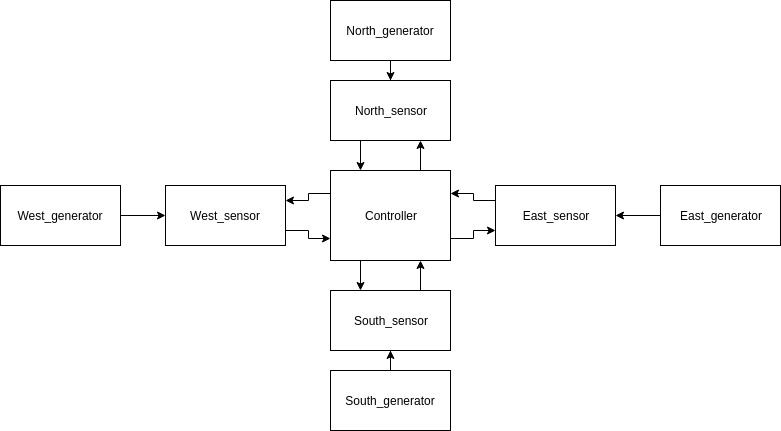
\includegraphics[width=1.5\linewidth]{system_img.jpg}
  }
  \caption{A boat.}
  \label{fig:boat1}
\end{figure}

\newpage%Explain the tests that we do and why we do them.
%Look what the lab has to be enabled to do according to the instructions and explain why our test dose that.

\section{How to run}
To run the system with the test files first make the project with < make -f MakeFile > and then <main.x fil1 file2 file3 file4 fileOut>. The files are input files for the directions with 0 representing no car and 1 represents a car. The last file is an output file. To compile the project to generate pseudo-random cars, use <make -f MakeFile_Random> and run <main.x> fs


%----------------------------------------------------------------------------------------


\end{document}
